\chapter{Deus et Eliseus Ascenderunt in Caelum}
\begin{center}
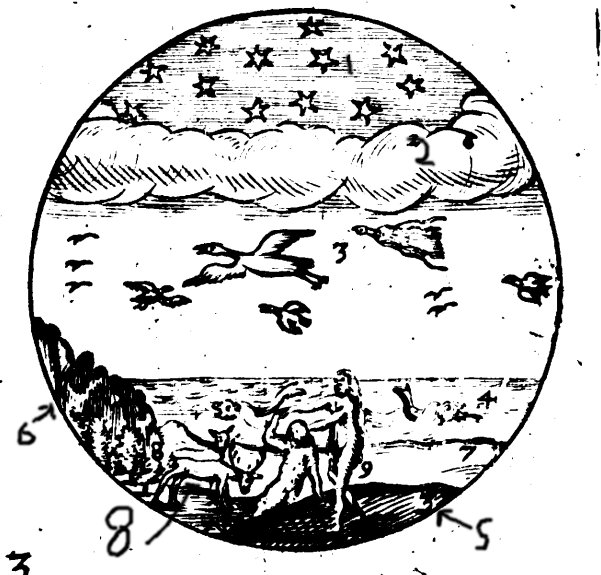
\includegraphics[scale=1.5]{World.png}
\end{center}

\section{Intended Audience}
This is intended for students who have completed Lectio 3 and 4 of Latin by the Natural Method and Chapter 4 of Lingua Latina Per Se Illustrata. There are 436 words in this chapter.

\section{Text}
Deus et Eliseus fīlius meus parvus ascendērunt in Caelum\footnote{\textbf{Caelum} = Heaven}. Quōmodo\footnote{\textbf{Quōmodo} = How, By What Means} Deus ascendit in caelum, sī sine corpore\footnote{\textbf{Sine corpore} = Without a body} et sine locō est? Deus incarnātiōnem\footnote{\textbf{Incarnātiōnem} = Incarnation} habet, quī ascendit in caelum et dēscendit ex caelō. Incarnātiō secundī\footnote{\textbf{Secundī} = of the second} hypostasis trīnitātis\footnote{\textbf{trīnitātis} = Trinity} est Iēsus Chrīstus. Ergō, Deus (In incarnātiōne) et Eliseus fuērunt in nūbibus\footnote{\textbf{Nūbibus} = In the Clouds}, quia ascendērunt in Caelō. Ēlīās etiam et Iēsus ascendērunt in caelum, sed Iēsus sōlus sedet ad manum\footnote{\textbf{Manum} = Hand} dexteram\footnote{\textbf{Dexteram} = Right} Deī. \par
In Caelō, Eliseus vīdit avēs\footnote{\textbf{Avēs} = Birds}, quae volāvērunt\footnote{\textbf{Volāvērunt} = They Flew} per nūbēs\footnote{\textbf{Nūbēs} = Through the Clouds}. Ubiubi\footnote{\textbf{Ubiubi} = Whereever} avis\footnote{\textbf{Avis} = Bird} volāvit, movet\footnote{\textbf{Movet} = It moves} āerem. Ubiubi Eliseus aspexit\footnote{\textbf{Aspexit} = He looked}, Eliseus vīdit avēs et nūbēs. Quid nōn vīdit Eliseus? Angelōs\footnote{\textbf{Angelōs} = Angels} nōn vīdit Eliseus. Cūr\footnote{\textbf{Cūr} = Why}? Suntne Angelī in Caelō cum Deō?  Angelī in caelō sunt. Caelum habet trēs\footnote{\textbf{Trēs} = Three} significātiōnēs\footnote{\textbf{Significātiōnēs} = Meanings}. Significātiō prīma\footnote{\textbf{Prīma} = First} est haec\footnote{\textbf{Haec} = This} \: Ubi sunt nūbēs et avēs et sōl et lūna. Significātiō secunda\footnote{\textbf{Secunda} = Second} \: Ubi sunt Angelī. Angelī nōn habent corpora nec locōs, sīcut Deus in essentiā, sed angelī in Caelō sunt. Tertia\footnote{\textbf{Tertia} = Third} significātiō est ubi est Deus, in aeternō. Angelī nōn sunt in aeternō, sed in aevō\footnote{\textbf{Aevō} = Aevum (The place which is described in subsequent sentences)}. Angelī in aevō sunt quia creātiōnēs immortālēs\footnote{\textbf{Immortālēs} = Immortal Beings(This is an adjective)} sunt sed nōn ex aeternō. Ubiubi es, Omnēs Angelī illīc\footnote{\textbf{Illīc} = There} sunt. Ubiubi es, Deus tenet tē in ente et cum tē est. Utut\footnote{\textbf{Utut} = However, in Whatevery Way} fēcistī, Deus cum tē est. Utut es, Deus cum tē est, quia Deus dēdit ēns tibi. \par
Dicāmus dē significātiōne prīmā. Caelum rotātur\footnote{\textbf{Rotātur} = Is rotated} et ambit\footnote{\textbf{Ambit} = it goes around} terram stantem\footnote{\textbf{Stantem} = Standing} in mediō\footnote{\textbf{In mediō} = In the middle}. Quid est "ambit". Sīcut terra ambit sōlem\footnote{\textbf{Sōlem} = Sun}, et nūbēs ambiunt terram. Iēsus fīlius Nun (Hic est Joshua anglice) ambit Jerichōnem septiēs\footnote{\textbf{Septiēs} = Seven Times}. Quid est "rotātur"? Terra rotātur et ambit Sōlem. Sōl nōn rotātur, sed stat\footnote{\textbf{Stat} = It stands}. Sōl, ubiubi est, fulget\footnote{\textbf{Fulget} = Shines} perpetuō\footnote{\textbf{Perpetuō} = Constantly}  in terrā. Sī nox\footnote{\textbf{Nox} = Night} in Eurōpā, diēs in Asiā. Nūbēs enim\footnote{\textbf{Enim} = For} sunt in caelō, tamen\footnote{\textbf{Tamen} = Still} sōl fulget, sed radiī\footnote{\textbf{Radiī} = The Rays} nōn sunt in terrā. Radius est lūx quam mīsit\footnote{\textbf{Mīsit} = It has sent} Sōl in terrā. Eliseus nōn vīdit sōlem, sī in nūbibus dēnsīs\footnote{\textbf{Dēnsīs} = Dense, Compact} est. Eliseus autem vīdit avēs, ergō nūbēs dēnsae nōn sunt, ergō Eliseus vīdit sōlem et radiōs eius. \par
In nocte est Tenebrae\footnote{\textbf{Tenebrae} = Darkness}. In nocte sunt Lūna\footnote{\textbf{Lūna} = Moon} et Stēllae\footnote{\textbf{Stēllae} = Stars}. Stēllae micant\footnote{\textbf{Micant} = They Twinkle} in caelō et scintillant\footnote{\textbf{Scintillant} = They Sparkle}. Nōn lūna scintillat, quia nōn Stēlla est, sīcut carmen\footnote{\textbf{Carmen} = Song} "Mīca, Micā Stēllam Parvam". Stēllae scintillant quia similis Scintillīs\footnote{\textbf{Scintillīs} = To Sparks} sunt. Scintilla est quae facit ignem, sīcut vir facit ignem cum scintillā. \par
In māne\footnote{\textbf{Māne} = In the Morning}, Sōl movet in Caelum. In vesperī\footnote{\textbf{Vesperī} = In the Evening}, sōl movet ex caelō. In māne, vir labōrat\footnote{\textbf{Labōrat} = He toils/works} cum aliīs hominibus\footnote{\textbf{Cum aliīs hominibus} = with other humans}. In māne, Stēllae nōn micant, nec Lūna splendet. In vesperī, Lūna splendet in Caelō, sed nōn stēllae. In vesperī, crepusculum\footnote{\textbf{Crepusculum} = Twilight} est. In māne, nōn est crepusculum, sed aurōra\footnote{\textbf{Aurōra} = Sunrise, Dawn} et dīlūculum\footnote{\textbf{Dīlūculum} = Daybreak}. In vesperī, Discipulī Chrīstī\footnote{\textbf{Discipulī Chrīstī} = Disciples of Christ (It's a plural and a genitive)} ōrant\footnote{\textbf{Ōrant} = They pray} Vesperās\footnote{\textbf{Vesperās} = Vespers (Evening Prayer)}. In māne, ōrant Laudēs\footnote{\textbf{Laudēs} = Lauds (Morning Prayer)}. Sōl fēcit lūcem, et ōrant Laudēs. Sōl fēcit tenebrās, et ōrant Vesperās. Deus amat\footnote{\textbf{amat} = He loves} Vesperās.\par